\documentclass[main]{subfiles}

\begin{document}


\chapter{Consideraciones sobre el controlador en el sistema real}
\label{chap:verificaciones_modelado}

A partir del simulador se encontr\'o una matriz de ralimentaci\'on que ofrece buenos resultados en cuanto a la robustez del sistema, el tiempo de respuesta del mismo y los sobretiros presentados en las diversas variables de estado. El pasaje del simulador al sistema real deber\'ia ser inmediato. Sin embargo no se obtuvieron los resultados esperados a priori.\\

Un primer problema detectado son las altas ganancias obtenidas en el simulador. El sistema real presenta polos de altas frecuencias que no son modelados. Al aumentar la ganancia del controlador estos polos comienzan a tener influencia sobre el comportamiento global del sistema. Se procedi\'o entonces a trabajar con una matriz de realimentaci\'on de menor norma. Para ello, se modific\'o la matriz \ref{eq:R} por:

\begin{equation}
R = \left(\begin{array}{cccc}
0.1 &0 &0 &0\\
0 &0.1 &0 &0\\
0 &0 &0.1 &0\\
0 &0 &0 &0.1
\end{array}\right)
\end{equation}

La matriz de realimentaci\'on obtenida tampoco ofrece resultados adecuados sobre el sistema real. La primer hip\'otesis planteada es que la caracter\'izaci\'on del sistema no es adecuada. A partir de aqu\'i se busca una forma alternativa de determinar los par\'ametros del sistema. El adecuado control de los \'angulos de Euler es fundamental para el equilibrio del sistema, por dicho motivo se comienza a trabajar en determinar en mejor forma los par\'ametros relevantes en las ecuaciones que influyen en estas variables de estado, haciendo part\'icular \'enfasis en el \'angulo de Pitch y en el de Roll.\\

Si restringimos el movimiento del cuadric\'optero a un giro segu\'un la direcci\'on $\vec{x}_q$ las ecuaciones que gobiernan al sistema linealizado en torno a las condiciones $\psi = \omega_{qx} = 0$ y $\omega_1 = \omega_3 =\omega_{hovering}$ son:
\begin{equation}
\label{eq:mod_psi}
\left(\begin{array}{c}
\dot{\psi}\\
\dot{\omega}_{qx}
\end{array}\right) = \left(\begin{array}{cc}
0 & 1\\
-\frac{MgL^\prime}{I_{xx}} & 0
\end{array}\right)\left(\begin{array}{c}
\psi\\
\omega_{wx}
\end{array}\right) + b\left(\begin{array}{cc}
0 & 0\\
1 & -1
\end{array}\right)\left(\begin{array}{c}
\omega_2\\
\omega_4
\end{array}\right)
\end{equation}

Donde
\begin{equation}
b =L\frac{2b_1\omega_{hovering}+b_2}{I_{xx}}
\end{equation}

La transferencia del sistema entre el \'angulo $\psi$ y la diferencia $\omega_2-\omega_4 (\Delta \omega)$ tiene la forma:

\begin{equation}
\label{eq:trans_psi}
H_{\psi}(s) = \frac{b}{s^2+\frac{MgL^\prime}{I_{xx}}}
\end{equation}

Analizando la respuesta al escal\'on de dicho \'angulo podemos obtener algunas relaciones que sirven para verificar las caracterizaciones realizadas. Inicialmente se tiene $\Delta \omega_i = -22.4 rad s^{-1}$, se aplica un escal\'on tal que $\Delta \omega_f = 13.5 rad s^{-1}$. En la figura \ref{fig:esc_psi} puede observarse la respusta del \'angulo $\psi$ a dicho escal\'on. En primer lugar cabe aclarar que el escal\'on se comporta acorde al modelo realizado ya que si as\'i fuese la oscilaci\'on no deber\'ia extinguirse, el decaimiento de la oscilaci\'on se debe a efectos no considerados en el set-up experimental, como por ejemplo la fricci\'on.\\

\begin{figure}
  \centering
 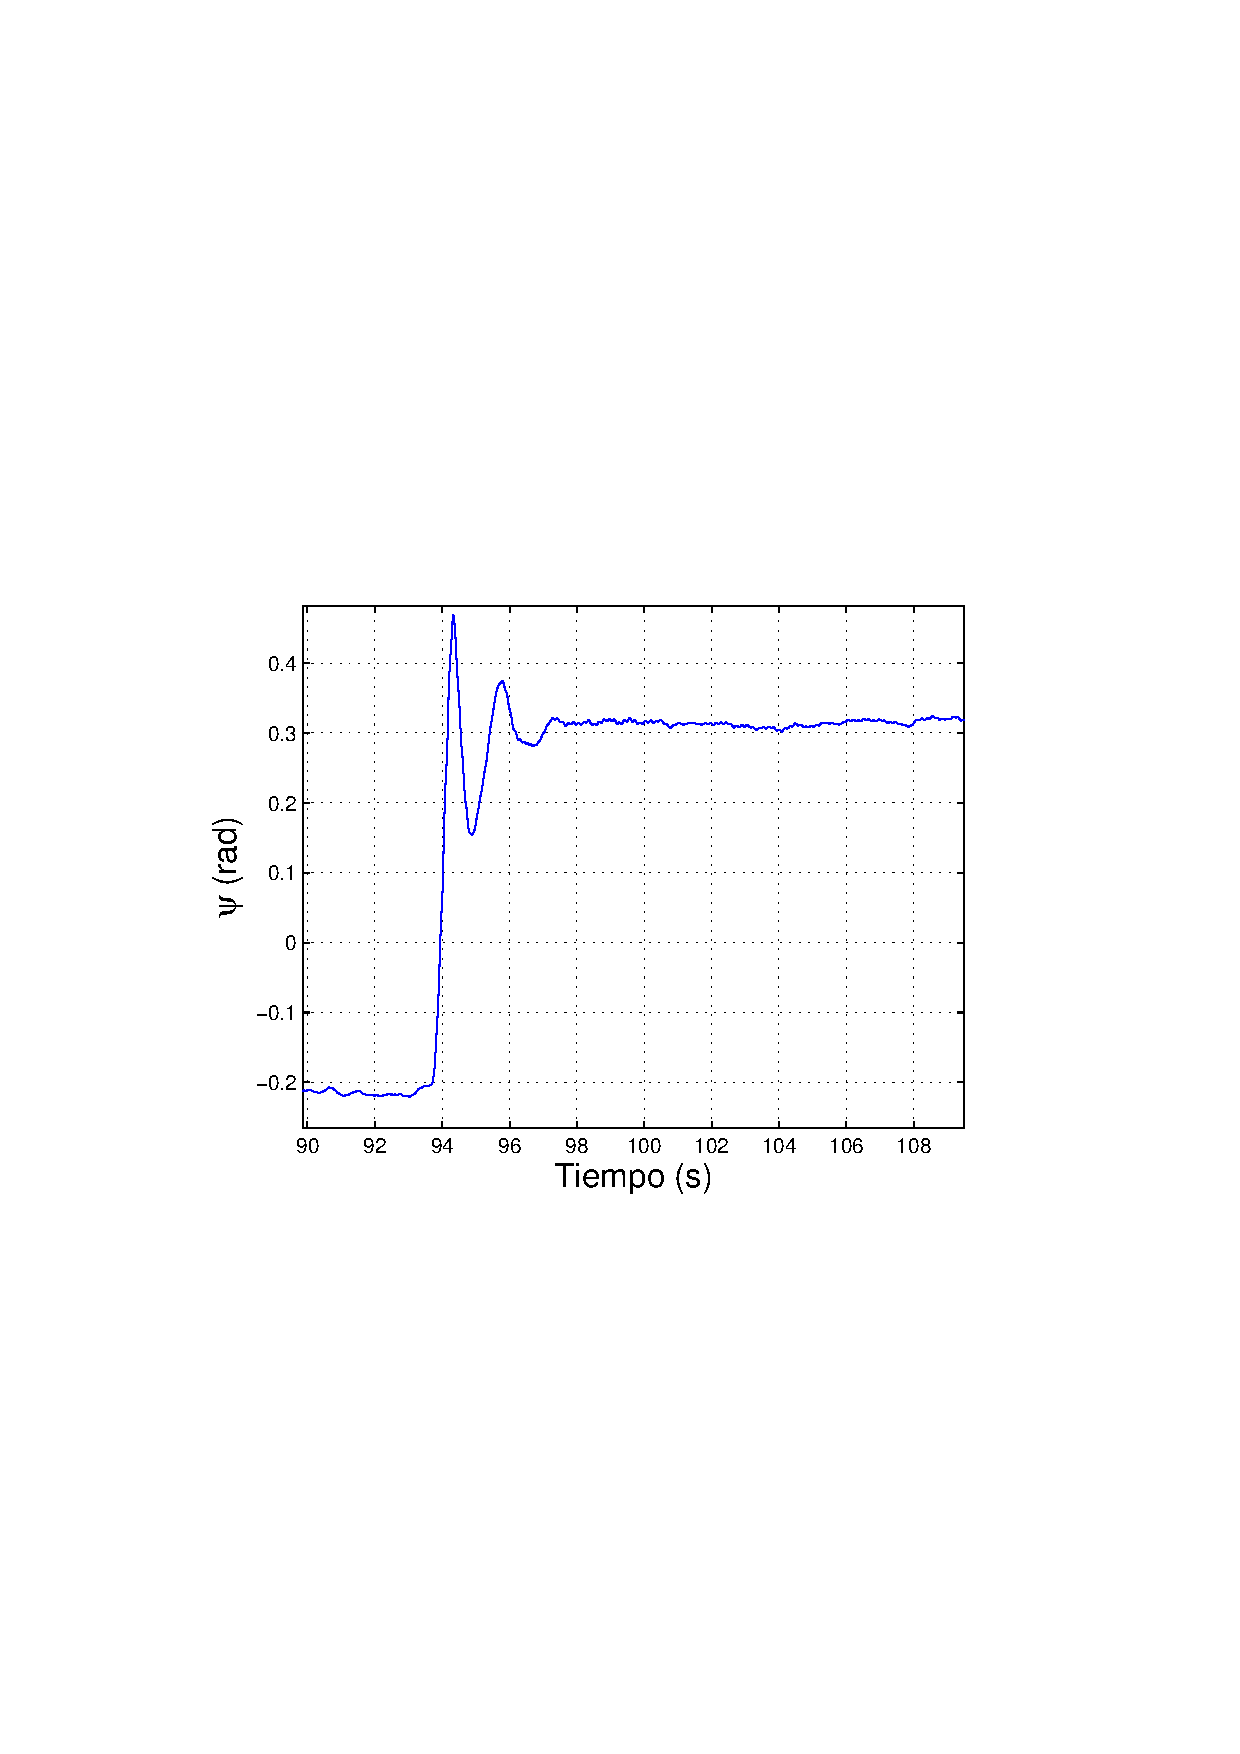
\includegraphics[width=0.8\textwidth]{./pics_verificacion/esc_psi}
  \caption{Respuesta al escal\'on del \'angulo $\psi$}
  \label{fig:esc_psi}
\end{figure}

De acuerdo a la figura \ref{fig:esc_psi} al aplicar un escal\'on en la entrada de $\Delta \omega_f - \Delta \omega_i = 35.9 rad s^{-1}$ el \'angulo $\psi$ varia desde $-0.22 rad$ alcanzando un valor en r\'egimen de $0.33 rad$, la variaci\'on total de dicho \'angulo es de $0.55 rad$. Por lo tanto la ganancia de la transferencia \ref{eq:trans_psi} es $\frac{0.55}{35.9}  \approx 0.015 s$. La ganancia de la transferencia puede expresarse adem\'as como $H_{\psi}(0)$. Por lo tanto se tiene que:

\begin{equation}
\frac{bI_{xx}}{MgL^\prime} = 0.015 s
\end{equation}

Por otra parte, si bien la respuesta al escal\'on experimental no se corresponde perfectamente con el modelo te\'orico, puede aproximarse el per\'iodo de las oscilaciones en el transitorio por el per\'iodo te\'orico $T_{teo} = \frac{2\pi}{\omega}$ donde $\omega = \sqrt{\frac{MgL\prime}{Ixx}}$. Bajo estas suposiciones el per\'iodo de acuerdo a la respuesta al escal\'on experimental es $1.2s$. Obtenemos entonces:

\begin{equation}
\omega = \frac{2\pi}{T} = \sqrt{\frac{MgL^\prime}{I_{xx}}}=5.23 s
\end{equation}

Si bien no es posible determinar absolutamente todos los par\'ametros del sistema si podemos calcular $b$ utilizando que:

\begin{equation}
b = H_{\psi}(0)\omega^2 = 0.41 s^{-1}
\end{equation}

Los valores calculados en func\'on de la primer caracterizaci\'on son:
\begin{itemize}
	\item $b = 0.35 s^{-1}$
	\item $\omega = \sqrt{\frac{MgL^\prime}{Ixx}} = 6.5s$
\end{itemize}

Los errores relativos entre los valores te\'oricos y experimentales para los par\'ametros $b$ y $\omega$ son del $14.6\%$ y del $24.32\%$ respectivamente. Estos errores no son para nada despreciables y pueden introducir diferencias significativas en el comportamiento del sistema en lazo cerrado simulado y el real. Modelando al sistema con los ``nuevos'' par\'ametros se obtienen resultados ampliamente satisfactorios como puede apreciarse en el cap\'itulo \ref{chap:test_control}\\

Intentaremos explicar la diferencia en el funcionamiento del sistema utilizando el lugar geom\'etrico de las raices. Consideremos el \'angulo de Roll, el controlador implementado es un controlador porporcional, integral y derivativo, el an\'alises lo realizaremos sin considerar el controlador integral. El funcionamiento del sistema tampoco era satisfactorio sin este t\'ermino con los primeros par\'ametros determinados y si lo fue, excepto por un error constante, con los ``nuevos'' par\'ametros.\\

La funci\'on de transferencia del controlador es:
\begin{equation}
C(s) = K_p+K_ds
\end{equation}
  
Por lo que la transferencia en lazo cerrado del sistema resulta en:
\begin{equation}
H_{\psi cl} (s)= \frac{H{\psi}(s)}{1+C(s)H{\psi}(s)}
\end{equation}

Los polos de dicho sistema son los ceros de \begin{equation}
1+C(s)H{\psi}(s)
\end{equation}

Buscar los ceros de dicha funci\'on es equivalente a buscar los puntos del plano complejo tales que:

\begin{equation}
1+\frac{K_pb}{s^2+bK_Ds+\frac{Mgd}{Ixx}} = 0
\end{equation}

Los polos de dicha funci\'on son:
\begin{equation}
\lambda_i = \frac{-bK_D \pm \sqrt{b^2K_D^2-4\frac{Mgd}{Ixx}}}{2}
\end{equation}

Seg\'un sea el signo del determinante tendremos un lugar geom\'etrico de las raices diferente. 
\end{document}